% Chapter3

\chapter{Grundlagen} \label{chapter:grundlagen}

%\begin{quotation}
%``The market is not an invention of capitalism. It has existed for centuries. It is an invention of civilization.``
%\begin{flushright}
%(Mikhail Gorbachev)
%\end{flushright}
%\end{quotation}

\section{Finanzwirtschaftliche Grundlagen}

% Alle Indikatoren beschreiben
% Quellen recherchieren
% Formel, wo m�glich
% Interpretation

\section{.NET-Framework}

% Was ist .NET
\subsection{Allgemein}

.NET ist ein Framework der Firma Microsoft, das eine Vielfalt an Sprachbibliotheken f�r eine gro�e Palette an Programmiersprachen zur Verf�gung stellt. Fr�her arbeiteten alle Programmiersprachen von Microsoft, wie bspw. C++, mit der WinAPI-32. Nun wurde dieses \gls{api} mit .NET durch ein sprachenunabh�ngiges, weitaus umfangreicheres Framework ersetzt. \cite{visualcsharp}\\
\\
Insgesamt wird die Nutzung des .NET-Frameworks von �ber 30 Programmiersprachen unterst�tzt. Die Richtlinien die eine Sprache einhalten muss, um als .NET-konform angesehen werden zu k�nnen, sind von Microsoft als \gls{cls} definiert worden. Zu den ber�hmtesten Vertretern solcher Sprachen Z�hlen C\#, F\#, Visual Basic .NET (VB.NET) und C++. \cite{visualcsharp}\\
\\
Zu den wichtigsten Features des .NET-Frameworks z�hlen die folgenden:
\begin{itemize}
\item \textbf{Objektorientierung} \\
	Das .NET-Framework ist zu 100\% objektbasiert. Das bedeutet, jegliche Elemente, sogar einfache Datentypen wie bspw. Integer, lassen sich auf Objekte zur�ckf�hren. Ja sogar die internen Zugriffe des Frameworks auf das darunterliegende Betriebssystem sind in Klassen gekapselt.
\item \textbf{Plattformunabh�ngigkeit} \\
	Anwendungen, die das .NET-Framework benutzen, werden �hnlich der \gls{jvm} erst zur Laufzeit in Maschinencode umgewandelt. Weiters ist die Spezifikation der von Microsoft benutzten Laufzeitumgebung, der sog. \gls{clr}, offen zug�nglich. Dadurch verlangt die Nutzung von .NET-Anwendungen also eine solche Umgebung, diese kann allerdings auch auf Plattformen portiert werden, die nicht Windows hei�en. So gibt es neben der propriet�ren Windows-Implementierung des .NET-Frameworks von Microsoft bspw. auch das \inline{Mono}-Projekt, mit dem .NET bereits erfolgreich auf Linux portiert werden konnte.
\item \textbf{Sprachenunabh�ngigkeit} \\
	Alle Komponenten des .NET-Frameworks k�nnen von jeder unterst�tzten Sprache problemlos verwendet werden. Das .NET-Framwork erm�glicht aber auch die Nutzung aller, in einer .NET-konformen Programmiersprache geschriebener Komponenten, in jeder anderen .NET-konformen Programmiersprache. So k�nnen zum Beispiel alle in C\# 2010 geschriebenen Klassen auch in F\# oder VB.NET genutzt und sogar abgeleitet werden.
\item \textbf{Speicherverwaltung} \\
	Die explizite Freigabe von nicht mehr ben�tigtem Speicher hat in der Vergangenheit schon zu vielen Problemen gef�hrt. Daf�r wurde mit dem .NET-Framework ein \inline{Garbage Collector} eingef�hrt, der dem Programmierer diese Aufgabe automatisch abnimmt. 
\item \textbf{Weitergabe} \\
	Auch die Weitergabe konnte deutlich vereinfacht werden. So k�nnen auf .NET basierende Sprachen einfach in eine .EXE- oder .\gls{dll}-Datei kompiliert und von jedem beliebigen Ordner aus ausgef�hrt werden. Eine .EXE-Datei ist dabei eine direkt ausf�hrbare Datei, deren Code bereits in einzelne Bytes umgewandelt wurde. \gls{dll}-Bibliotheken werden im folgenden Punkt erl�utert. \cite{visualcsharp}
\end{itemize}
% Was sind DLLs

\section{C\#-Grundlagen}

% Was ist C# (Microsoft)
% objektorientiert
\subsection{Allgemein}

Die Programmiersprache C\# wurde von der Firma Microsoft entwickelt und gilt als einer der wichtigsten Sprachen, die das .NET-Framework benutzen. C\# ist eine objektorientierte Programmiersprache mit einer fundamentalen Sprachsyntax. Mit diesen Eigenschaften eignet sie sich auch perfekt f�r die Nutzung von .NET. \cite{visualcsharp}\\
\\
Die Sprachsyntax von C\# ist der von Java sehr �hnlich. C\# wurde erstmals mit dem Ziel entwickelt, eine bessere, funktionsreichere Sprache zu entwickeln, die Java abl�sen k�nnte, trotzdem allerdings dessen Vorteile nutzt. Auch die allgemeine Struktur einer Klasse sowie der Aufbau simpler Anweisungen (if, for, while, etc.) sind quasi ident zu ihren �quivalenten in Java. \cite{visualcsharp}\\
\\
Eine C\#-Anwendung kann grunds�tzlich als Konsolenanwendung oder mit einer graphischen Oberfl�che (\gls{gui}) ausgef�hrt werden. Zur Realisierung einer solchen \gls{gui} werden ebenfalls mehrere Mechanismen zur Verf�hung gestellt. Zum einen gibt es die mittlerweile veraltete direkte M�glichkeit der Realisierung mit WinForms, einer API, die direkt in die Sprache integriert ist. Zum anderen hat Microsoft die \gls{wpf} entwickelt, die im folgenden Abschnitt \ref{wpf} genauer erl�utert wird. \cite{visualcsharp} \\
\\
Im folgenden sollen nun alle wichtigen Technologien der Sprache C\# beschrieben werden, die im Zuge dieses Projektes zum Einsatz gekommen sind.
% WPF
	% MVVM
	% XAML-GUI
	% GUI-Bindung
\subsection{Windows Presentation Foundation} \label{wpf}

Mit Version 3.0 des .NET-Frameworks wurde wie bereits erw�hnt zus�tzlich zur altbew�hrten WinForms-Variante, eine neue Variante integriert um Benutzeroberfl�chen einfach zu implementieren. Diese hei�t \gls{wpf}. \cite{visualcsharp}\\
\\
Das wichtigste Merkmal von \gls{wpf} gegen�ber anderen Methoden zur \gls{gui}-Erstellung ist, dass bei \gls{wpf} die Programmlogik nach strengsten Richtlinien von der Beschreibung der Oberfl�che trennt. Diese Beschreibung der Oberfl�che erfolgt mittels einer speziellen Version der normalen \gls{xml}, der \gls{xaml}. Mit dieser Sprache werden alle \gls{gui}-Komponenten, erzeugt und in die entsprechende Position gebracht. Bei \gls{wpf} wird allerdings trotzdem auch eine \gls{api} f�r den Zugriff auf \gls{xaml}-\gls{gui}-Komponenten innerhalb der Programmlogik bereit gestellt. Bei der Erstellung eines \gls{wpf}-Projektes, bekommt man automatisch ein MainWindow.xaml-File. Ein solches \gls{xaml}-File das lediglich einen Button als \gls{gui} anzeigt, w�rde nun in etwa so aussehen: \cite{visualcsharp}\\
\\
\begin{verbatim}
<Window x:Class="Wpf1Application1.MainWindow"
    xmlns="http://schemas.microsoft.com/winfx/2006/xaml/presentation"
    xmlns:x="http://schemas.microsoft.com/winfx/2006/xaml"
    Title="MainWindow" Height="350" Width="525">
    <Grid>
    	<Button Name="button1">Button</Button>
    <\Grid>
</Window>
\end{verbatim}

Hierbei werden zuerst die n�tigen von Microsoft definierten \gls{xaml}-Namespaces angegeben. Anschlie�end werden ein Titel (der ganz oben im Fenster angezeigt wird) und die Gr��e des Fensters angegeben, dass sp�ter unseren Button beinhalten soll. Danach wird ein einfaches Grid-Layout mit einem Button mit dem Text "Button" gezeichnet. Ab Microsoft Visual Studio 2008, wird auch ein \gls{wpf}-\gls{gui}-Builder bei der Installation mitgegeben, mit dem man diese \gls{xaml}-Dateien einfach mit graphischer Oberfl�che erstellen kann. \cite{visualcsharp}\\
\\
Zu der MainWindow.xaml-Datei wird auch noch eine weitere Datei mit dem Namen MainWindow.xaml.cs erstellt. Diese wird auch als \textit{Code-Behind}-Datei bezeichnet und beinhaltet den Teil der Programmlogik der direkt mit der graphischen Oberfl�che verkn�pft ist. M�chte man also bspw. die Logik implementieren, die beschreibt was bei einem Klick auf den Button passiert, m�sste man dies in eben dieser MainWindow.xaml.cs-Datei durchf�hren. \cite{visualcsharp}

\subsection{MVVM}
Als \gls{mvvm} wird ein Entwicklungsmuster (Design-Pattern) verstanden, dass sehr oft in Verbindung mit der Implementierung von \gls{wpf}-Oberfl�chen eingesetzt wird. Dabei werden die einzelnen Aufgaben einer Anwendung mit graphischer Oberfl�che in drei Teile aufgeteilt. Es gibt nun ein View, ein Model und ein ViewModel. Deren Interaktion kann in der Abbildung \ref{fig:mvvm} sehr sch�n nachvollzogen werden. \cite{msdn-mvvm}\\

\begin{figure}[h]
	\centering
		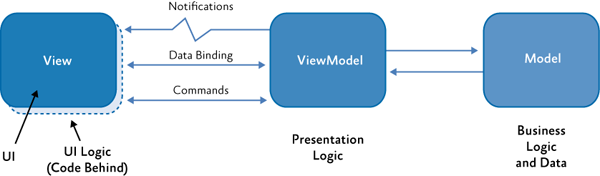
\includegraphics[width=0.90\textwidth]{graphics/grundlagen/mvvm.png}
	\caption{Aufbau von \gls{mvvm}}
	\label{fig:mvvm}
\end{figure}

Zuerst gibt es da also den View-Teil. Der View beschreibt das Aussehen der \gls{gui}. Im Optimalfall befindet sich um View ausschlie�lich ein Konstruktor mit einem Methodenaufruf InitializeComponents(), der die \gls{gui} �ber das \gls{xaml}-File aufbaut. Sollen allerdings komplexere graphisch aufwendigere Elemente oder Animationen in der grafischen Oberfl�che gezeichnet werden, kann diese Logik im View-Teil implementiert werden. Im View sollte allerdings nie Logik programmiert werden die man einem Unit-Testing unterziehen muss.\\ Wie der Abbildung \ref{fig:mvvm} entnommen werden kann, kommunziert der View nicht direkt, sondern ausschlie�lich �ber Commands, Notifications oder Data Binding mit dem ViewModel. Auf Commands wird hier nicht n�her eingegangen, Data Binding und Notifications k�nnen allerdings im folgenden Abschnitt \ref{databinding} gefunden werden. \cite{msdn-mvvm}\\
\\
Der ViewModel-Teil kapselt nun die Presentationslogik und die von der \gls{gui} ben�tigten Daten. Das ViewModel hat keinen direkten Zugriff auf den View und wei�t daher nichts �ber dessen Implementierung. Das ViewModel kann bspw. �ber die Verwaltung von Daten, die mittels Data Binding an den View weitergegeben werden mit diesem kommunizieren. Nebenbei bemerkt, m�ssen alle Daten die �ber Data Binding an den View weitergegeben werden sollen ausschlie�lich im ViewModel gespeichert werden. Das ViewModel beschreibt also welche Funktionalit�t die \gls{gui} anbieten soll und das View, wie diese angezeigt wird. Das ViewModel fungiert au�erdem quasi als Mittelmann zwischen dem View und dem Model und kann dabei bspw. noch die Daten aus dem Model so vereinfachen, dass der View diese leichter verarbeiten kann. \cite{msdn-mvvm}\\
\\
Das Model ist nun die eigentliche Gesch�fts- oder Programmlogik und die damit verbundenen allgemeinen Daten. Hierbei handelt es sich um eine ganz normale Gesch�ftslogik wie in anderen Anwendungen auch, nur dass noch einmal speziell Wert darauf gelegt werden sollte die einzelnen Codest�cke nicht Task-spezifisch zu implementieren, um die einzelnen St�ck sp�ter m�glicherweise an anderen Stellen wiederverwenden zu k�nnen. Au�erdem besteht das Model entgegen dem View und dem Viewmodel meist aus vielen einzelnen Model-Klassen, die alle mit dem selben ViewModel kommunizieren. M�chte das Model auch mit dem View interagieren gibt es auch hier die M�glichkeit Notifications zu benutzen.\cite{msdn-mvvm}

\subsection{Data Binding} \label{databinding}

Das Data Binding (auch: Datenbindung) erm�glicht \gls{gui}-Komponenten den Zugriff auf Daten, die sie anzeigen k�nnen. In WinForms war die Datenbindung auch schon integriert, lediglich war man mit den damaligen Methoden auf wenige Controls beschr�nkt. Mit \gls{wpf} ist man dies nun nicht mehr. Daten k�nnen hiermit n�mlich direkt aus einer der folgenden Datenquellen entnommen werden \cite{visualcsharp}:

\begin{itemize}
	\item ViewModel
	\item Eigenschaften anderer Komponenten
	\item \gls{xml}-Datei
	\item Collections
	\item Datenbanken
	\item etc.
\end{itemize} \cite{visualcsharp}

Zur Nutzung von Data Binding sind nun zwei Klassen wichtig, DataContext und Binding. Der DataContext ist die Datenquelle von der die Daten bezogen werden sollen. Dieser DataContext ist au�erdem ein Attribut jedes \gls{gui}-Elements und muss gesetzt werden, damit Bindungen funktionieren. M�chte man nun den DataContext setzen sollte man aber aufpassen und ihn im �bergeordneten Container (z.B. dem MainWindow) setzen, denn davon profitieren alle untergeordneten Komponenten dieses Conatiners und der DataContext muss nict �berall gesetzt werden. Das Binding-Objekt beschreibt nun die Binung zwischen einer Datenquelle und einer bindenden Komponente. Das Binding wird meist im \gls{xaml}-Code geschrieben, es besteht allerdings selbstverst�ndlich auch die M�glichkeit sie innerhalb des C\#-Codes zu erzeugen. \cite{visualcsharp}\\
\\
Das einfachste Beispiel f�r eine Bindung k�nnte nun in etwa so aussehen:

\begin{verbatim}
<Window x:Class="Wpf1Application1.MainWindow"
    xmlns="http://schemas.microsoft.com/winfx/2006/xaml/presentation"
    xmlns:x="http://schemas.microsoft.com/winfx/2006/xaml"
    Title="MainWindow" Height="350" Width="525">
    <Window.DataContext>
    	<local:MainViewModel x:Name="mainViewModel" />
    </Window.DataContext>
    <StackPanel>
    	<TextBox Name="txtOben" Height="50" FontSize="16"></TextBox>
    	<TextBox Name="txtUnten" Height="50" Background="AliceBlue" FontSize="16">
    		<Binding ElementName="txtOben" Path="Text" />
    	</TextBox>
    </StackPanel>
</Window>
\end{verbatim} \cite{visualcsharp}

Zuerst wird hier der \textit{DataContext} auf das ViewModel gesetzt. Dies w�re hier zwar noch nicht notwendig, da keine Bindung auf ein Property aus dem ViewModel erfolgt, es zeigt allerdings die angesprochene Funktionsweise und wird im n�chsten Beispiel von Bedeutung sein. Danach werden zwei \textit{TextBoxen} erstellt von denen die Text-Variable der unteren eine Bindung auf die Text-Variable der oberen besitzt. Dadurch wird der Text der unteren \textit{TextBox} automatisch an den Text der oberen \textit{TextBox} angepasst, falls sich dieser �ndert. Eine Bindung in dieser Art k�nnte aber auch auf jedes andere Attribute der \textit{TextBoxen} (z.B. Gr��e, Schriftart, etc.) angewendet werden. Dazu m�sste lediglich der \textit{Path} der Bindung ge�ndert werden. \cite{visualcsharp}\\
\\
Eine etwas kompliziertere Bindung ist die auf ein Property aus dem ViewModel. Dazu muss man zuerst im ViewModel ein Property erzeugen und dessen setter-Methode f�r die Nutzung von Notifications implementieren. Das Property, das die Lieblingsfarbe einer Person speichert, k�nnte dann in etwa so aussehen \cite{msdn-mvvm}:

\begin{verbatim}
public class MyViewModel : INotifyPropertyChanged
{
    private string favoriteColor;
    public event PropertyChangedEventHandler PropertyChanged;
    ...
    public string FavoriteColor
    {
        get { return this.favoriteColor; }
        set
        {
            if (value != this.favoriteColor)
            {
                this.favoriteColor = value;
                if (this.PropertyChanged != null)
                {
                    this.PropertyChanged(this,
                          new PropertyChangedEventArgs("FavoriteColor"));
                }
            }
        }
    }
}
\end{verbatim} \cite{msdn-mvvm}

Hierbei wird einfach eine globale Variable (\textit{favoriteColor}) mit einem Property (\textit{FavoriteColor}) versehen, das die setter-Methode so implementiert hat, dass ein \textit{PropertyChangedEvent} gesendet wird, sobald der Wert der Lieblingsfarbe ge�ndert wird. Dies ist notwendig, wenn man das Property an ein \gls{gui}-Element binden will, da sich das \gls{gui}-Element, sonst im Falle einer �nderung der Lieblingsfarbe nicht aktualisieren w�rde. M�chte man dieses Property nun im \gls{xaml}-Code an ein \gls{gui}-Element binden, muss man lediglich das Folgende schreiben:

\begin{verbatim}
<Window x:Class="Wpf1Application1.MainWindow"
    xmlns="http://schemas.microsoft.com/winfx/2006/xaml/presentation"
    xmlns:x="http://schemas.microsoft.com/winfx/2006/xaml"
    Title="MainWindow" Height="350" Width="525">
    <Window.DataContext>
    	<local:MainViewModel x:Name="mainViewModel" />
    </Window.DataContext>
    <StackPanel>
    	<TextBox Name="favoriteColorTextBox" Height="50" FontSize="16">
    		<Binding Path="FavoriteColor" />
    	</TextBox>
    </StackPanel>
</Window>
\end{verbatim}

Diesmal ist die Definition des ViewModels als \textit{DataContext} notwendig. Aus diesem wird n�mlich einfach in der Bindung das \textit{FavoriteColor}-Property aufgerufen. Schon steht zu jeder Zeit die aktuelle Lieblingsfarbe aus dem ViewModel in der \textit{TextBox}.
% Charting-Library (.NET)
\lstset{style=sharpc}
\subsection{Microsoft Chart Controls} \label{charting}

Die Microsoft Charts Controls Library ist eine sehr umfangreiche Bibliothek, die es erm�glicht in WinForms-Anwendungen oder auf Webseiten mit ASP.NET Charts und Diagramme zu zeichnen. Die M�glichkeiten sind derma�en umfangreich, dass es im Folgenden nur Sinn macht, die Funktionen zu erl�utern, die f�r die Darstellung finanzieller Charts erheblich sind. Zu den Hauptfeatures z�hlen daher \cite{msdn-charting}:

\begin{itemize}
\item \textbf{Charttypen} \\
	Es werden 35 verschiedene Charttypen unterst�tzt, dabei alles von normalen Liniencharts bis zu Bar- und Candlestick-Charts zur Darstellung von Aktiendaten.
\item \textbf{Skalierbarkeit} \\
	Es k�nnen unendlich viele Daten, Chart-Areas (Bereiche innerhalb eines Charts), Bemerkungen (z.B. Pfeile), etc. innerhalb eines Charts angezeigt werden. Daher k�nnen bspw. Aktiendaten und deren \glspl{ma} in einer ChartArea angezeigt werden. Zus�tzlich k�nnte man eine weitere ChartArea erg�nzen um bspw. einen \gls{macd}-Verlauf direkt unter den Aktiendaten zu zeichnen.
\item \textbf{Daten} \\
	Es werden Unmengen an M�glichkeiten zur Verwaltung der Daten innerhalb eines Charts, wie z.B. Data Binding, zur Verf�gung gestellt. Au�erdem k�nnen die Daten des Charts exportiert, oder zum Speichern serialisiert werden. 
\item \textbf{Aussehen} \\
	Weiters k�nnen sowohl zweidimensionale als auch dreidimensionale Charts erstellt werden, die alle sehr simpel und sch�n dargestellt werden. Die k�nnen zudem auch zur Laufzeit noch weiter manipuliert werden und die WinForms-Version bietet sogar M�glichkeiten zum interaktiven Zoomen und Scrollen f�r den User. (Auf Webseiten mit ASP.NET werden keine interaktiven Funktionen f�r den Benutzer der Website angeboten.) 
\end{itemize} \cite{msdn-charting}

\subsubsection{Nutzung mit WPF} \label{winformshost}

Leider ist momentan noch keine Version f�r die Verwendung mit \gls{wpf} erh�ltlich, man kann diese Einschr�nkung allerdings umgehen indem man einen sog. \textit{WinFormsHost} erstellt. Dies ist ein \gls{wpf}-\gls{gui}-Element, das WinForms-Elemente so kapselt, dass sie in \gls{wpf} genutzt werden k�nnen. Dieses Element mit einem \textit{MSChart} kann so erstellt werden:

\begin{lstlisting}[label=MSChart in einer WinFormsHost-Umgebung,caption=MSChart in einer WinFormsHost-Umgebung]
<WindowsFormsHost Name="WfHost" Grid.Row="0">
	<MSChart:Chart x:Name="MyWinformChart">
	    <MSChart:Chart.ChartAreas>
	        <MSChart:ChartArea Name="MainArea"/>
	    </MSChart:Chart.ChartAreas>
	</MSChart:Chart>
</WindowsFormsHost>
\end{lstlisting}

Hier wurde au�er dem primitiven \textit{MSChart} auch gleich eine \textit{ChartArea} hinzugef�gt. Eine \textit{ChartArea} ist ein Bereich innerhalb des Charts (hier der gesamte Bereich des Charts), in dem eine Funktion gezeichnet werden kann. Damit dieses WinFormsHost-Element allerdings funktioniert m�ssen f�r das gesamte \textit{Window} noch folgende Namespaces erg�nzt werden (diese Assemblies m�ssen nat�rlich auch als Verweis zum Projekt hinzugef�gt werden):

\begin{lstlisting}[label=Namespaces f�r MSChart und WinFormsHost,caption=Namespaces f�r MSChart und WinFormsHost]
xmlns:wf="clr-namespace:System.Windows.Forms;assembly=System.Windows.Forms"
xmlns:MSChart="clr-namespace:System.Windows.Forms.DataVisualization.Charting;assembly=System.Windows.Forms.DataVisualization"
xmlns:wfi="clr-namespace:System.Windows.Forms.Integration;assembly=WindowsFormsIntegration"
\end{lstlisting}

\subsubsection{Darstellung einfacher Graphen}

Nachdem eine leere \textit{ChartArea}, in die ein Graph gezeichnet werden kann, bereits im \gls{xaml} erzeugt wurde, muss man im C\#-Code nur noch das \textit{Chart} suchen, in das gezeichnet werden soll und eine \textit{Series} erstellen. In diese Series werden dann die Daten eingespeist, die gezeichnet werden soll. Wenn man nun auch noch einen Typ f�r den Graphen konfiguriert wird dieser auch schon in der \textit{ChartArea} angezeigt. Um bspw. eine Sinusfunktion darzustellen m�sste man nun folgenden Code schreiben: \cite{msdn-charting}

\begin{lstlisting}[label=Erstellung einer Series,caption=Erstellung einer Series]
//Lookup des bereits im XAMl-Code definierten Charts
Chart chart = this.FindName("MyWinformChart") as Chart;

//Erstellen der Series
Series sinus = new Series("Sinus");

//Berechnung einer Sinuskurve und speichern der
//errechneten Daten in die Series
for (double i = 0; i <= 7.5; i += 0.2)
	sinus.Points.AddXY(i, Math.Sin(i));

//Definieren des Zeichentyps als normale Linie
sinus.ChartType = SeriesChartType.FastLine;
 
// Hinzufuegen des Graphs zum Chart
chart.Series.Add(sinus);
\end{lstlisting} \cite{mschart-grundlagen}

In diesem Beispiel wurde jeder Punkt des Sinus einzeln berechnet und zur \textit{Series} hinzugef�gt. Dies k�nnte man nat�rlich auch mit jeder anderen Datenquelle wie zum Beispiel einer Liste machen, in dem man jeden Wert einzeln hinzuf�gt. \cite{msdn-charting}

\subsubsection{Finanzielle Berechnungen} \label{finfor}

Die Microsoft Chart Controls Library bietet allerdings nicht nur M�glichkeiten zur einfachen Darstellung von Daten. Denn sie beinhaltet ein Framework aus �ber 50 veschiedenen statistischen und finanziellen Formeln zur automatischen Berechnung und Darstellung spezieller Werte. \cite{msdn-charting}\\
\\
Die wichtigsten Formeln in der \textit{FinancialFormula}-Sammlung der MS Chart Controls sind:

\begin{itemize}
\item Bollinger B�nder
\item \gls{cci}
\item diverse \glspl{ma}
\item \gls{macd}
\end{itemize} \cite{msdn-charting}

Im Code w�rde der Einsatz von \textit{FinancialFormula} so aussehen:

\begin{lstlisting} [label=Berechnung eines WMA mit FinancialFormula,caption=Berechnung eines WMA mit FinancialFormula]
chart.DataManipulator.FinancialFormula(FinancialFormula.WeightedMovingAverage, 90, "Data", "FinFor");
\end{lstlisting} \cite{msdn-charting}

Dieser Aufruf erzeugt einen \gls{ma} der L�nge 90. Dazu holt er sich die Daten aus der Series ''\textit{Data}'', berechnet den \gls{ma} und schreibt die errechneten Daten in die \textit{Series FinFor}. Damit diese Berechnung m�glich ist muss die \textit{Series FinFor} bereits zuvor erzeugt und die \textit{Series Data} ebenfalls bereits zuvor erzeugt auch wirklich mit Daten gef�llt sein. \cite{msdn-charting}
% C# Tuples
\lstset{style=sharpc}
\subsection{C\# Tupel}

Ein Tupel ist prinzipiell eine Ansammlung von Werten. Dabei kann es beliebig viele Werte mit verschiedenen Datentypen haben. Eben diese Anzahl und die dazugeh�rigen Datentypen m�ssen allerdings schon im Vorhinein festgelegt werden, wenn das Tupel erzeugt wird. Ein \inline{Tuple} in C\# k�nnte bspw. so aussehen \cite{cs-tuple}:

\begin{lstlisting} [label=Erstellung eines Tuples,caption=Erstellung eines Tuples]
Tuple<int, bool> tuple = new Tuple<int, bool>(1, true);
\end{lstlisting}

Dabei handelt es sich um ein sehr einfaches \inline{Tuple}, das lediglich einen Integer-Wert zu einem dazugeh�rigen Boolean-Wert speichert. Ein \inline{Tuple} ist eine Klasse, in der direkt Werte gespeichert werden. Deshalb muss er einen separaten Ort im Heap allokieren. \cite{cs-tuple} Dies bedeutet, dass bspw. ein Tupel mit zwei Werten in der Erstellung wesentlich l�nger ben�tigt als ein \inline{KeyValuePair}, es aber sp�ter in der Nutzung eine deutlich h�here Performance aufweist. \cite{tuple-performance} Au�erdem k�nnen durch diese Tatsache die Datentypen der Felder des Tupels nach dessen Erstellung absolut nicht mehr ge�ndert werden, was das \inline{Tuple} eigentlich mehr einer \inline{struct} �hneln l�sst. \cite{cs-tuple}\\
\\
In der Praxis werden selten einzelne Tupel verwendet. Es ist allerdings oft von Vorteil eine Liste aus Tupeln zu erzeugen, wenn man quasi eine \inline{Map} (bzw. ein \inline{Dictionary}) mit mehreren Werten oder anderen Datentypen ben�tigt. So k�nnen z.B. Aktienpreis-Bars als Tupel aus einem \inline{TimeStamp} und Feldern f�r Open, High, Low und Close realisiert werden. Daraus kann dann eine Liste erstellt werden, um die Bars ad�quat speichern zu k�nnen.
% Speichern
% LINQ

\section{F\#-Grundlagen}

% F# in Verbindung mit anderen Sprachen
% Was sind DLLs
% Pattern-Matching
% Piping-Operator
% Funktionsweise von Arrays, Lists, Sequences
% Datenstruktur-Performance (Messung, EMA)
